\section{Timing layers for single particles}

Now let us discuss the kinematic regions for the TOF measurements in relation to
either SM particles or BSM particles. 
 
For an estimation of the separation power between different mass hypotheses, we will
calculate the mass and momentum for which one can achieve separation significance higher than $3\sigma$ (or $p$-val$<0.03$)
If we have two particles with masses $m$ and a reference (fixed) mass $m_F$, the $3\sigma$ separation can be 
achieved assuming this condition  \cite{Cerri:2018rkm}:

\begin{equation}
\frac{L}{c \sigma_{\textsc{TOF}}}\left|\sqrt{1+\frac{m^2}{p^2}} - \sqrt{1+\frac{m_F^2}{p^2}}\right| > 3
\label{eqTOF}
\end{equation}
where $p$ is the momenta of particles, $L$  is the length of the particle trajectory, and $\sigma_{TOF}$ is the
resolution  of the timing layer that measures the TOF.

Figure~\ref{fig:singleparticles} shows the $3\sigma$ separation from the pion
mass hypothesis ($m_F=m_{\pi}$) using the same procedure as discussed  in \cite{Cerri:2018rkm}. The 
calculations are performed for several options for the resolution of the timing layer, from 10~ps to 1~ns,
as a function of the travel length $L$ and the momenta. For a 20~ps detector and  for a typical travel 
distance of $L\sim 0.2$~m from the interaction point to the 
electromagnetic calorimeter, neutrons (and protons) can be separated from the pion hypothesis up to 7~GeV. The separation of $K-$mesons can be performed up to 3~GeV.
This momentum range should be sufficient for reliable particle identification in a wide range 
of physics studies, especially if such identification is used for jets that are dominated
by this momentum range of separate particles.
For a detector  with 1~ns, the separation can only be possible  up to  300 -- 500~MeV. This is below  than a typical
minimum transverse momentum of 0.5 -- 1~GeV for particles considered for high-energy proton colliders .
Therefore, a timing layer with 1~ns resolution cannot effectively be used for particle identification in such experiments.

\begin{figure}
\begin{center}
   \subfigure[Neutrons] {
   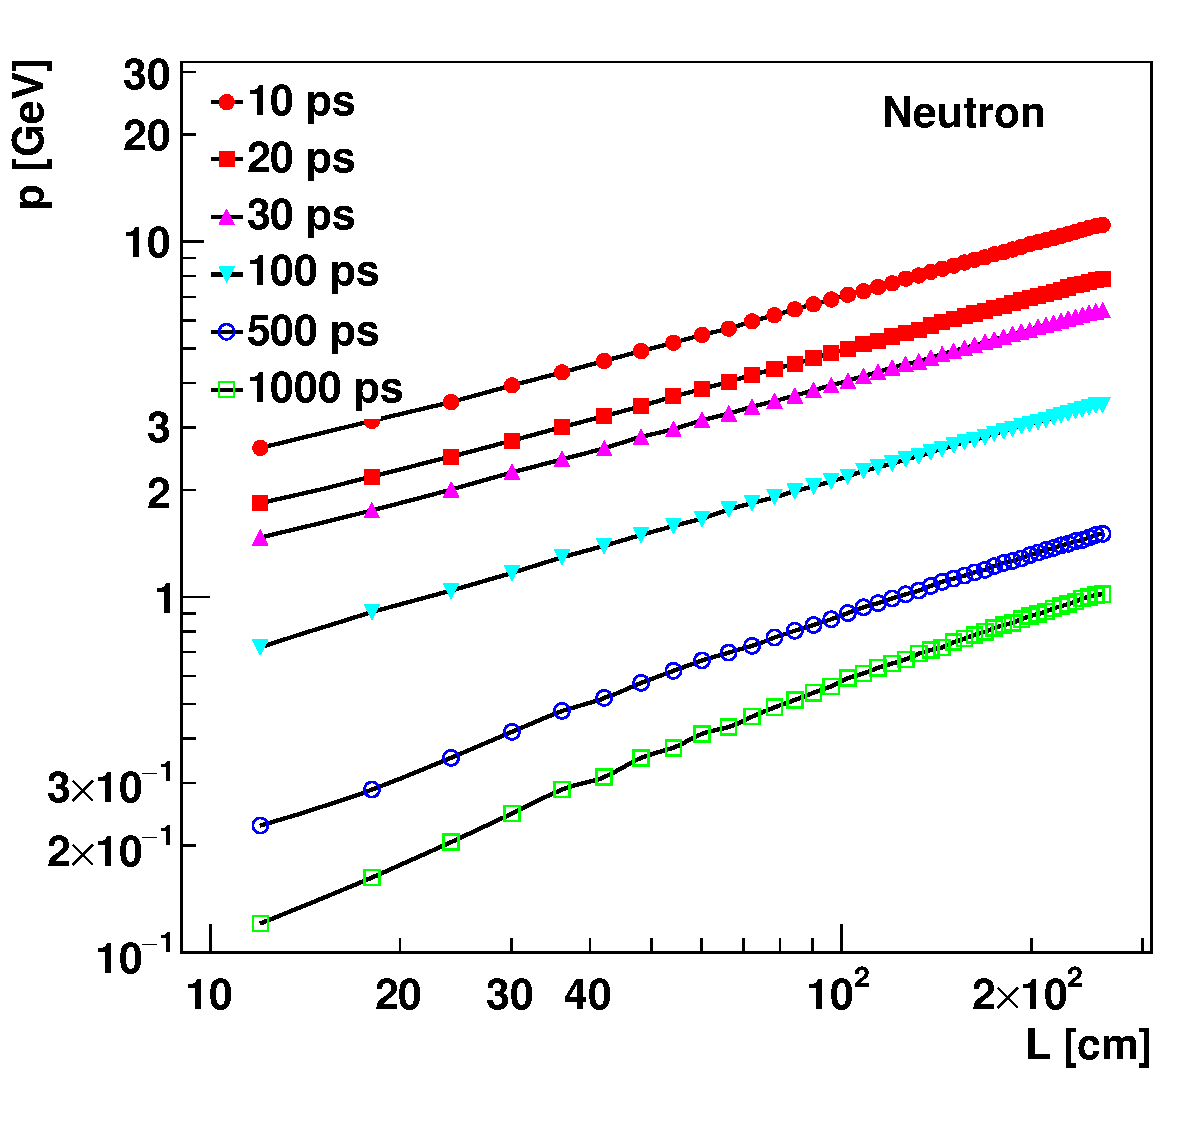
\includegraphics[width=0.45\textwidth]{time_flight_length_neutron.pdf}
   }
      \subfigure[$K$-mesons] {
   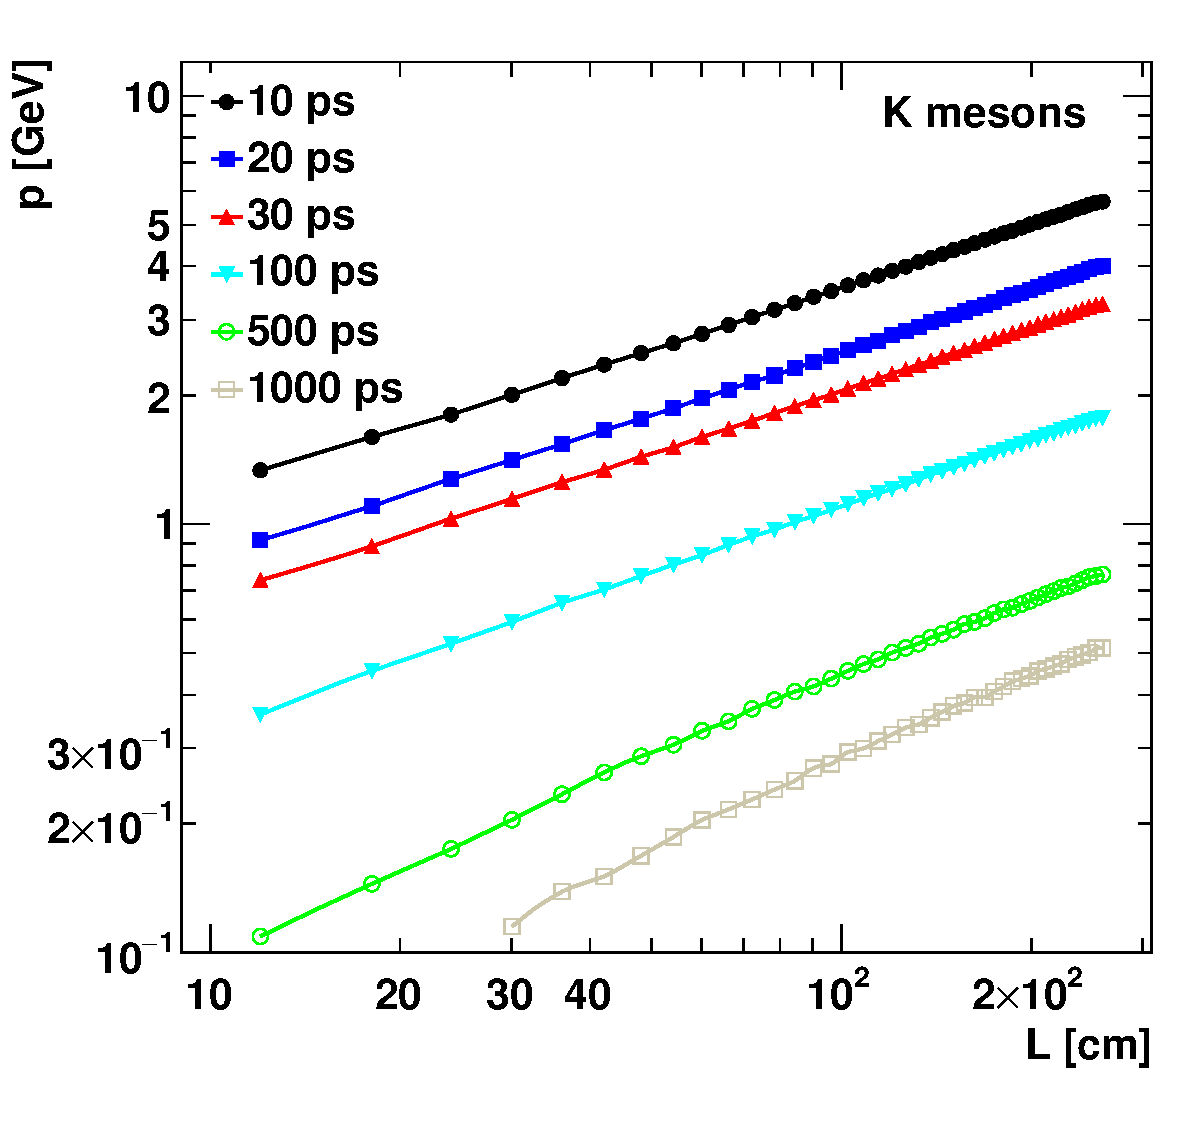
\includegraphics[width=0.45\textwidth]{time_flight_length_kion.pdf}\hfill
   }
\end{center}
\caption{
The $3\sigma$ separation from the pion mass for neutrons and $K$-mesons as a function of the distance and the momenta.
}
\label{fig:singleparticles}
\end{figure}


\begin{figure}
\begin{center}
   \subfigure[for $L=2$~m] {
   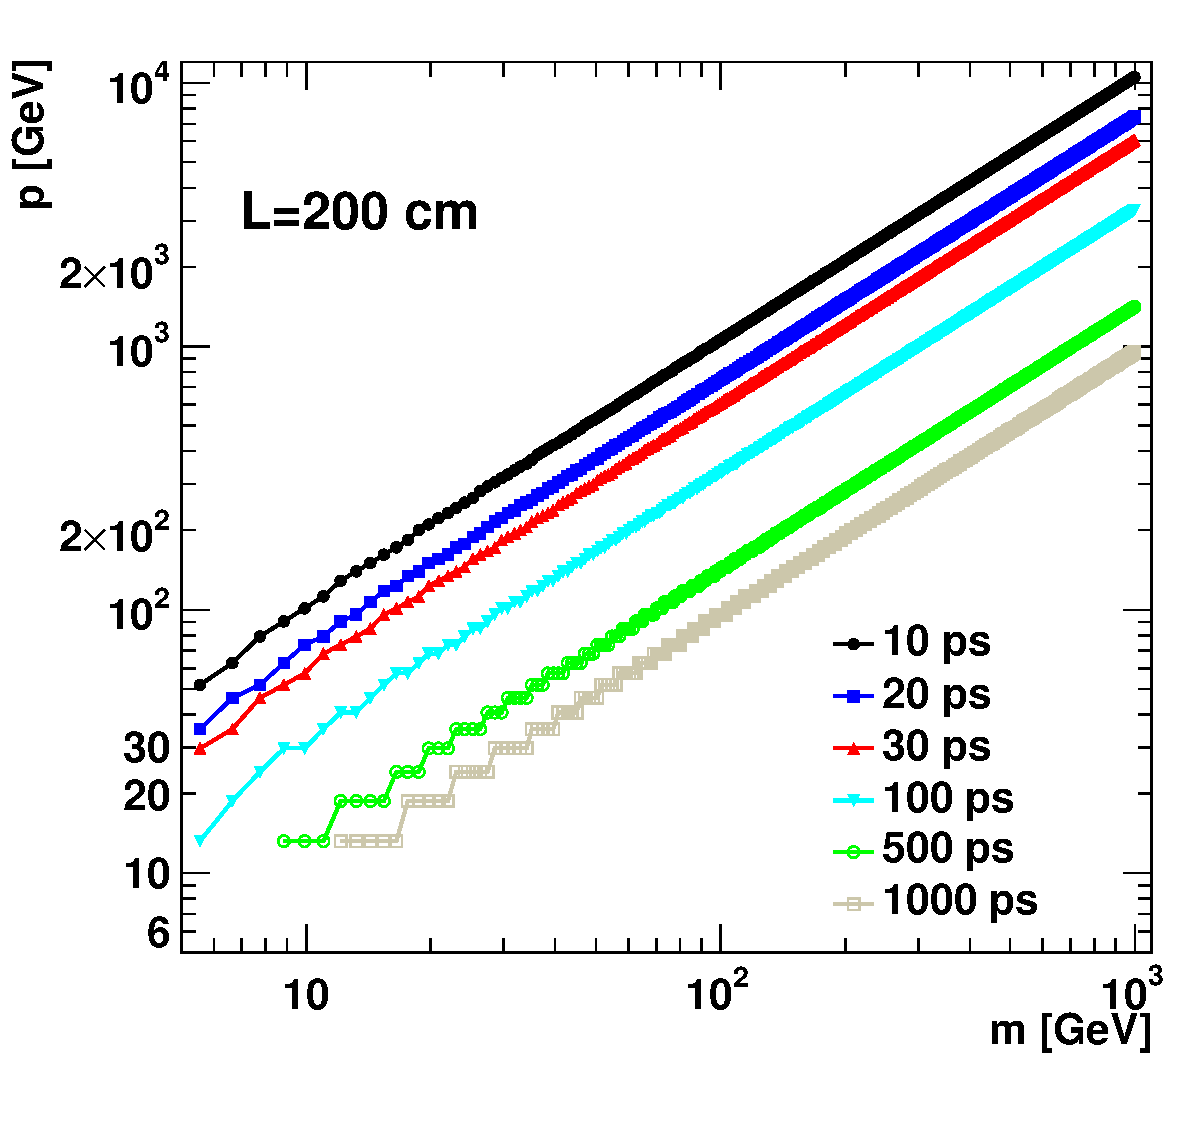
\includegraphics[width=0.45\textwidth]{time_flight_200.pdf}
   }
   \subfigure[for $L=0.2$~m] {
   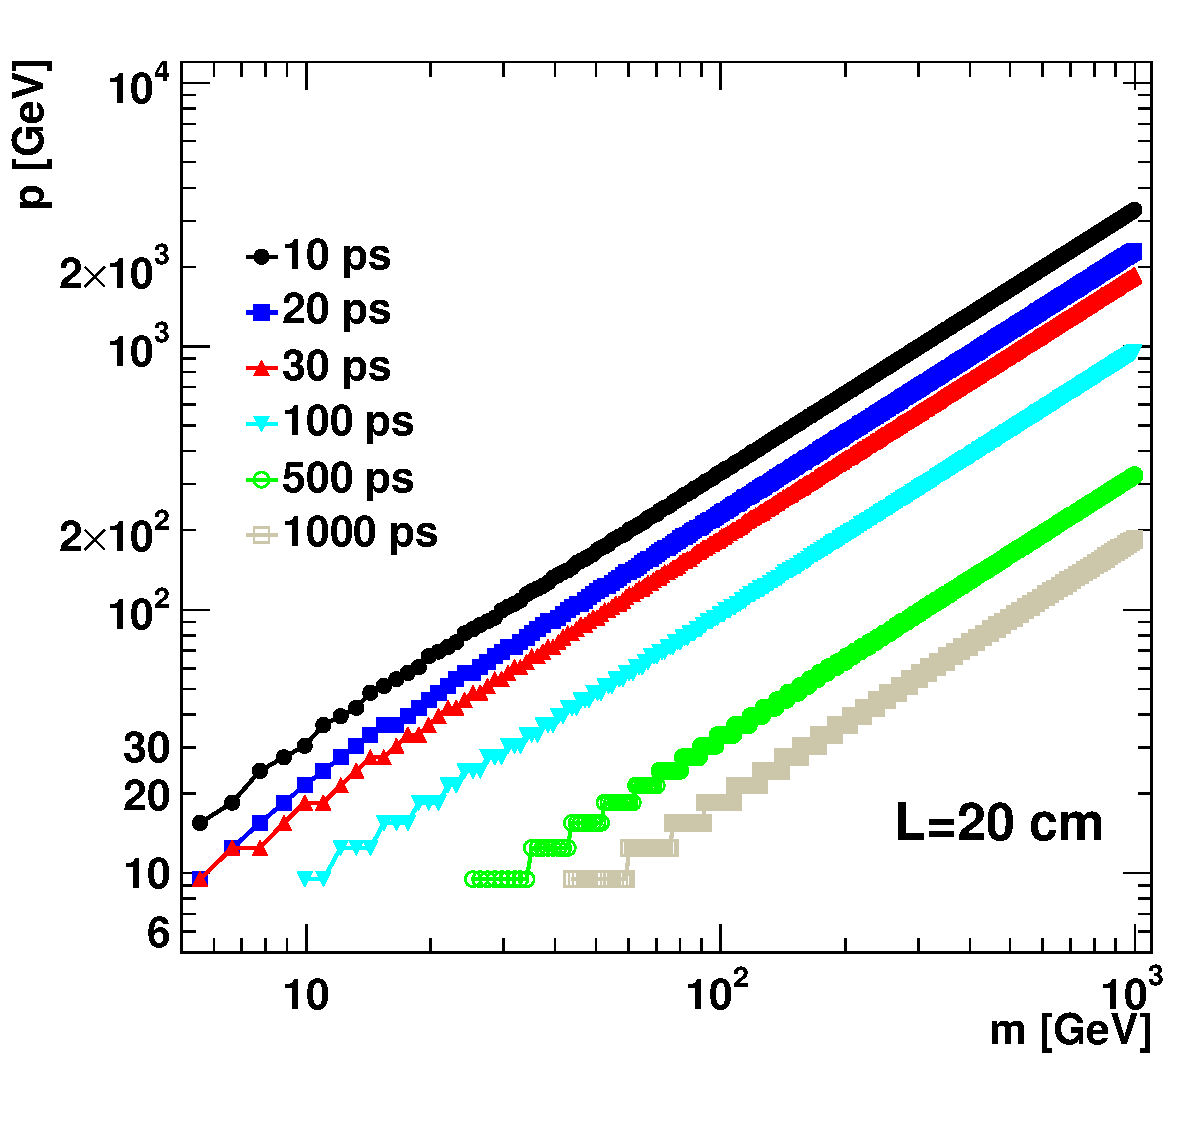
\includegraphics[width=0.45\textwidth]{time_flight_20.pdf}\hfill
   }
\end{center}
\caption{
The $3\sigma$ identification for heavy particles assuming timing layers with different resolutions for TOF, and using $L=2$~m and $L=0.2$~m.
The first value is a typical distance
from the vertex to the first layer ($TL_1$), while the second value is the typical  distance
between two timing layers enclosing an electromagnetic calorimeter, assuming a typical calorimeter
based on the silicon technology.
}
\label{fig:signgleBSM}
\end{figure}


Having discussed a rather obvious case of identification of neutrons (or protons) and the $K$-mesons from the pion hypothesis,
let us turn to the BSM searches for heavy particles.
The most abundant SM background for light BSM  particles from primary interactions are protons and neutrons.
Other stable particles, that can be produced mainly in 
detector material (or from the interaction in the beam pipe) 
and detected by calorimeter are deutrons and $\alpha$ particles (composed from two protons and two neutrons). 
Although the rate of $\alpha$ particles sh be low since such particles can easy be stopped by detector material,
it is not impossible that residual rate may still  represent background for BSM searches that have a lower production rate.  
Therefore, we will choose  $m_F=m_{\alpha}\simeq 3.73$~GeV  for Eq.~\ref{eqTOF} and evaluate the
$3\sigma$ separation for a wide range of masses and momentum.
For most future experiments the distance between the 
interaction point and the first layer of the electromagnetic calorimeter is 
$L=1.5-2.5$~m. For a representative purpose, we will use $L=2$~m and consider 0.2~m for the  separation
distance between the TL2 and TL1 timing layers.

Figure~\ref{fig:signgleBSM} shows the particle identification power for different choices of the timing layer resolution
and the distance $L=L_1$ to the first timing layer (see Fig.~\ref{fig:eff_rad}).
For $L=L_1=2$~m, one can be see that a stable heavy particle with a mass of 100~GeV can be reconstructed up to 
400~GeV assuming a 20~ns timing layer,
but only up to 50~GeV using the standard 1~ns calorimeter.

One can also consider a  measurement that does not involve a priory knowledge  of the vertex, thus can be better
designed for neutral particles in collisions with large pile-up (multiple number of vertexes).  
In the case the TOF is measured between the two layers, TL1 and TL2, assuming a successful spacial match of the hits.

The identification power in the case when the distance between TL2 and TL1 is 0.2~m is shown in Figure~\ref{fig:signgleBSM}(b).
For a 100~GeV stable particle, the identification is possible up to about 100~GeV. The standard calorimeter with
$1$~ns resolution can perform the identification up to $20$~GeV. 

